\documentclass[tikz,border=5mm]{standalone}
\usepackage{pgfplots}
\pgfplotsset{compat=1.18}

\begin{document}

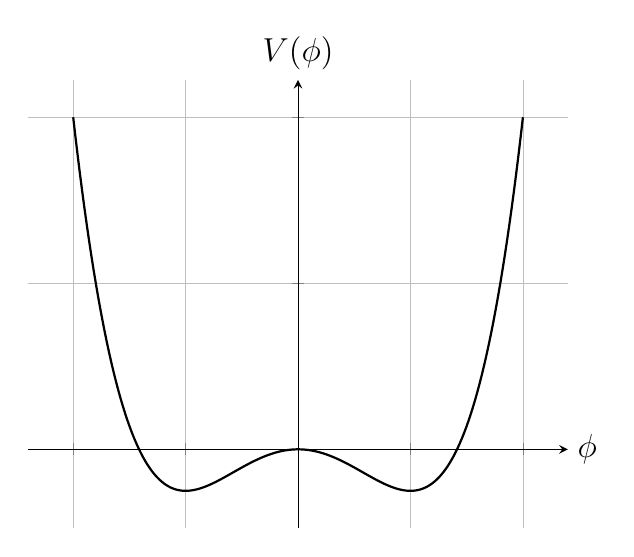
\begin{tikzpicture}
    \begin{axis}[
        axis lines=middle,
        xlabel={$ \phi $},
        ylabel={$ V(\phi) $},
        enlargelimits,
        every axis x label/.style={at={(current axis.right of origin)}, anchor=west},
        every axis y label/.style={at={(current axis.above origin)}, anchor=south},
        xlabel style={font=\large},
        ylabel style={font=\large},
        xtick={-2,-1,0,1,2}, % Define x-axis ticks
        ytick={-1,0,1,2,3},  % Define y-axis ticks
        xticklabels=\empty, % Hide x-axis labels
        yticklabels=\empty, % Hide y-axis labels
        grid=both, % Add both major and minor grid lines
        minor grid style={dotted}, % Minor grid style as dotted
        major grid style={solid, gray!50}, % Major grid style as solid and lighter gray
        grid style={line width=0.2pt} % Grid line thickness
    ]
        % Plot the potential
        \addplot[domain=-2:2, samples=200, thick, black] {-0.5*x^2 + 0.25*x^4};
    \end{axis}
\end{tikzpicture}

\end{document}
